%%%%%%%%%%%%%%%%%%%%%%%%%%%%%%%%%%%%%%%%%%%%%%%%%%%%%%%%%%%%%%%%%%%
%                                                                 %
%                            CHAPTER FIVE                         %
%                                                                 %
%%%%%%%%%%%%%%%%%%%%%%%%%%%%%%%%%%%%%%%%%%%%%%%%%%%%%%%%%%%%%%%%%%%

\chapter{ONTOLOGY AND TAXONOMY VERSIONING}

This chapter extensively uses the GCMD Keywords data set to study methods of determining the extent of change in a data set.
The keywords have a long sequence of versions, allowing trends to be observed over the course of releases.

\section{Creating the Versioning Graph}

The Global Change Master Directory maintains and releases the different versions of their keyword list.
From this, it can be concluded that each edition shares provenance and can be used in the same workflow step.
This conclusion is further justified as each keyword concept uses the same Unique Resource Identifier (URI) across versions.
The identifiers also act as an ideal key in the version mapping.
While additions and invalidations are simple to identify using these keys, modifications are not since a change in the key would result in completely different object.
Instead, we look at the immediately broader concept.
Each keyword uses the concepts \textit{skos:Broader} and \textit{skos:Narrower}, where skos refers to the Simple Knowledge Organization System ontology name space, to form a tree hierarchy with the broadest concept "Science Keywords" forming the root.
A modification would then result if a concept moved to a different place in the hierarchy.
This would result in the removal of a child node from the parent and a different broader concept for the child, meaning two modifications occur.
However, in this project, only the child is recorded since it is the concept that moves around in the hierarchy.
Versioning graphs for each comparison was generated by extracting JSON-LD from the corresponding change log, and entering the triples into a Fuseki triple store.

\section{Quantifying Change}

The GCMD group migrated their keywords into a centralized Keyword Management System (KMS) as of June 12, 2012.
Each subsequent keyword release has been supplied an identifier by the management group and the add, invalidate, and modify counts between each transition are presented in Figure \ref{GCMDC1}.
The query used to extract the counts is found in Listing \ref{gcmd_list}.
Notice the sharp spike in adds and invalidates when transitioning from version 8.4.1 to 8.5.
Not only should a small transition not produce changes of this magnitude, but the data sets size is on the order of the recorded invalidates.
In addition, no modifications are revealed, and even the root node "Science Keywords" has been invalidated.
Further investigation of the root word reveals that the name space for the keywords has changed from HTTP to HTTPS.
Since the identifiers are unique, this means they no longer refer to the same object after the protocol change.
This results in the whole data set being invalidated and a new data set being added.
However, the dot decimal identifier only indicates a minor change, demonstrating a difference between the producer's perceived divergence and the actual change.
To provide context, NASA mandated a transition to secure protocols, and the group changed the named space to ensure the URIs remained resolvable.

\begin{figure}%[b]
	\centering
	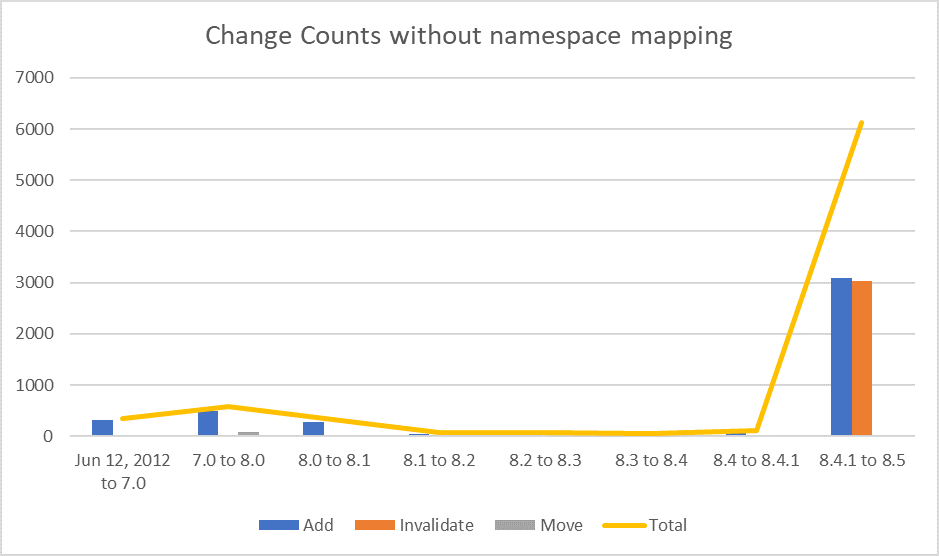
\includegraphics[scale=1]{figures/GCMDChart1.png}
	\caption{Add, Invalidate, and Modify counts in Version 8.5.  The counts show change magnitudes and indicate that major and minor changes differ by orders of magnitude.}
	\label{GCMDC1}
\end{figure}

\hfill \break
\begin{lstlisting}[language=SPARQL, caption=This query compiles the counts for each subclass of Change in a GCMD versioning graph,label=gcmd_list]
PREFIX vo:<http://orion.tw.rpi.edu/~blee/VersionOntology.owl>
PREFIX rdfs:<http://www.w3.org/2000/01/rdf-schema#>

SELECT ?p (COUNT (DISTINCT ?s) as ?count)
{
	?s a ?p .
	?p rdfs:subClassOf vo:Change .
} GROUP BY ?p
\end{lstlisting}

That the data producers did not perceive this change in name space to be a major modification can be demonstrated by accounting for the change and recounting.
In the modified mapping, HTTP and HTTPS identifiers are treated the same.
Differences in change magnitudes become much clearer after controlling for the altered name space in Figure \ref{GCMDC2}.
All revisions are dominated by additions, but major version changes have counts around 300 to 500 while minor revisions are an order of magnitude smaller.
This includes the transition from version 8.4.1 to 8.5.
From the identifier scheme and the change counts, it is clear that the keyword management team expected only minor changes in the keywords.
This analysis demonstrates that relying on data producers to name their versions using the dot decimal identifiers based on their perceived change also relies on their perceiving the intended utilization of their data set by all their users.
The count results seem to indicate that they can differentiate between major and minor revisions, but it also shows that current version labels may not capture all the change within a transition.


\begin{figure}%[b]
	\centering
	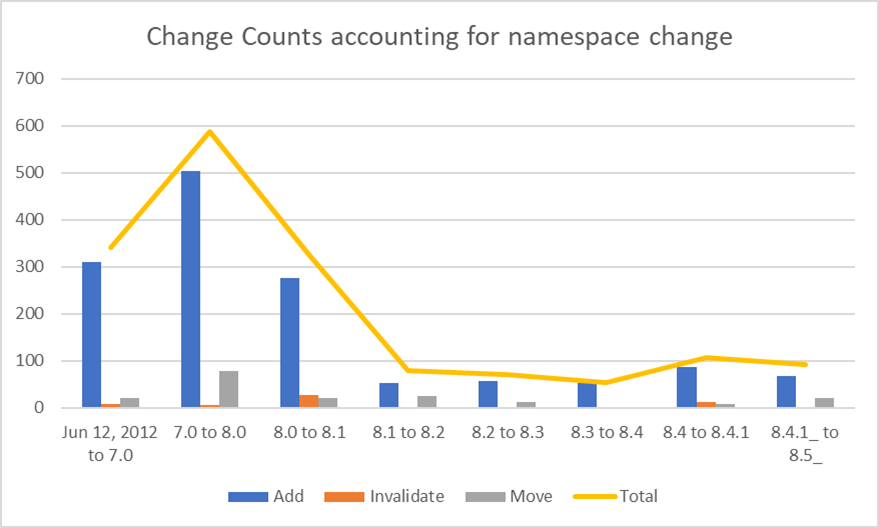
\includegraphics[scale=1]{figures/GCMDChart2.png}
	\caption{Add, Invalidate, and Modify counts ignoring the namespace changes in Version 8.5.  The counts show change magnitudes appropriate for the identifier.}
	\label{GCMDC2}
\end{figure}